\documentclass[11pt]{article}

\usepackage{amsmath}
\usepackage{tabularx}
\usepackage{subcaption} 
\usepackage{textcomp}
\usepackage{caption}
\usepackage{graphicx}
\usepackage{hyperref}
\usepackage[top=0.8in, bottom=0.8in, left=0.8in, right=0.8in]{geometry}
% Add other packages here %

\usepackage{epstopdf}
\epstopdfDeclareGraphicsRule{.tif}{png}{.png}{convert #1 \OutputFile}
\AppendGraphicsExtensions{.tif}

% Put your group number and names in the author field %
\title{\bf{Classifying Roof Material From Drone Imagery} \\
 An Approach to the Open AI Caribbean Challenge}
\author{Johannes Leonhard Ruether}


% N.B.: The report should not be longer than 3 pages 

\begin{document}
	\maketitle
	
	\section{Introduction (Context and Challenges)}
	
	\subsection{Context}
	
	Regions like the Carribean are regularly hit by rainstorms, floods or earthquakes. Despite being so prone, many houses in those areas are unable to withstand these natural hazards due to poor construction quality. This exposes their inhabitants to a great risk of becoming homeless during the next natural disaster. 
	
	International programs such as the World Bank's Global Program for Resilient Housing are making attempts to retrofit houses to the natural forces they are exposed to. In these large and often informal settlements it is difficult to assess which houses pose especially high risks due to their construction or are damaged and need repair. Exploring these areas on the ground is time-consuming and costly. 
	This is why the possibilities of image processing for automatic recognition of vulnerable houses on the basis of drone imagery are explored. Such a technology could assist building inspectors and narrow down large areas to those that are worth a closer inspection on the ground. 
	The material that a roof are made up of is a central indicator of how well a house is prepared against natural disasters. Therefore, classifying roof material from aerial images is a key step to identify precarious houses. \\
	
	\subsection{Open AI Challenge}
	
	The above reasons led to the initiation of the \textit{Open AI Caribbean Challenge: Mapping Disaster Risk from Aerial Imagery}, which was conducted between October and December 2020 on \textit{drivendata.org}.	
	This report describes an approach to solve this challenge.\\
	
	\subsection{Previous Work}
	
	In many applications, the identification of roofs is considered useful. Roof segmentation is often done with LiDAR data, as presented in \cite{Chen2012}. Other papers such as \cite{Soman2019} have successfully attempted roof segmentation using only drone imagery, which is less costly. This step will become relevant for the task at hand. The approach discussed in this report however uses images of roofs that have already been segmented.\\
	
	The identification of roof defects has been addressed in previous works, e.g. \cite{Yudin2018}, in which water stagnation on roofs is measured. Multiple patents (e.g. \cite{Shreve2017}) describe the use of aerial images to evaluate damage on individual roofs for insurance purposes. To my best knowledge, academic works on roof material and condition classification from drone imagery on a large scale have however not been published. 
	
	\section{Data Description}
	
	\subsection{Images}
		
	\begin{figure}
		\centering		
		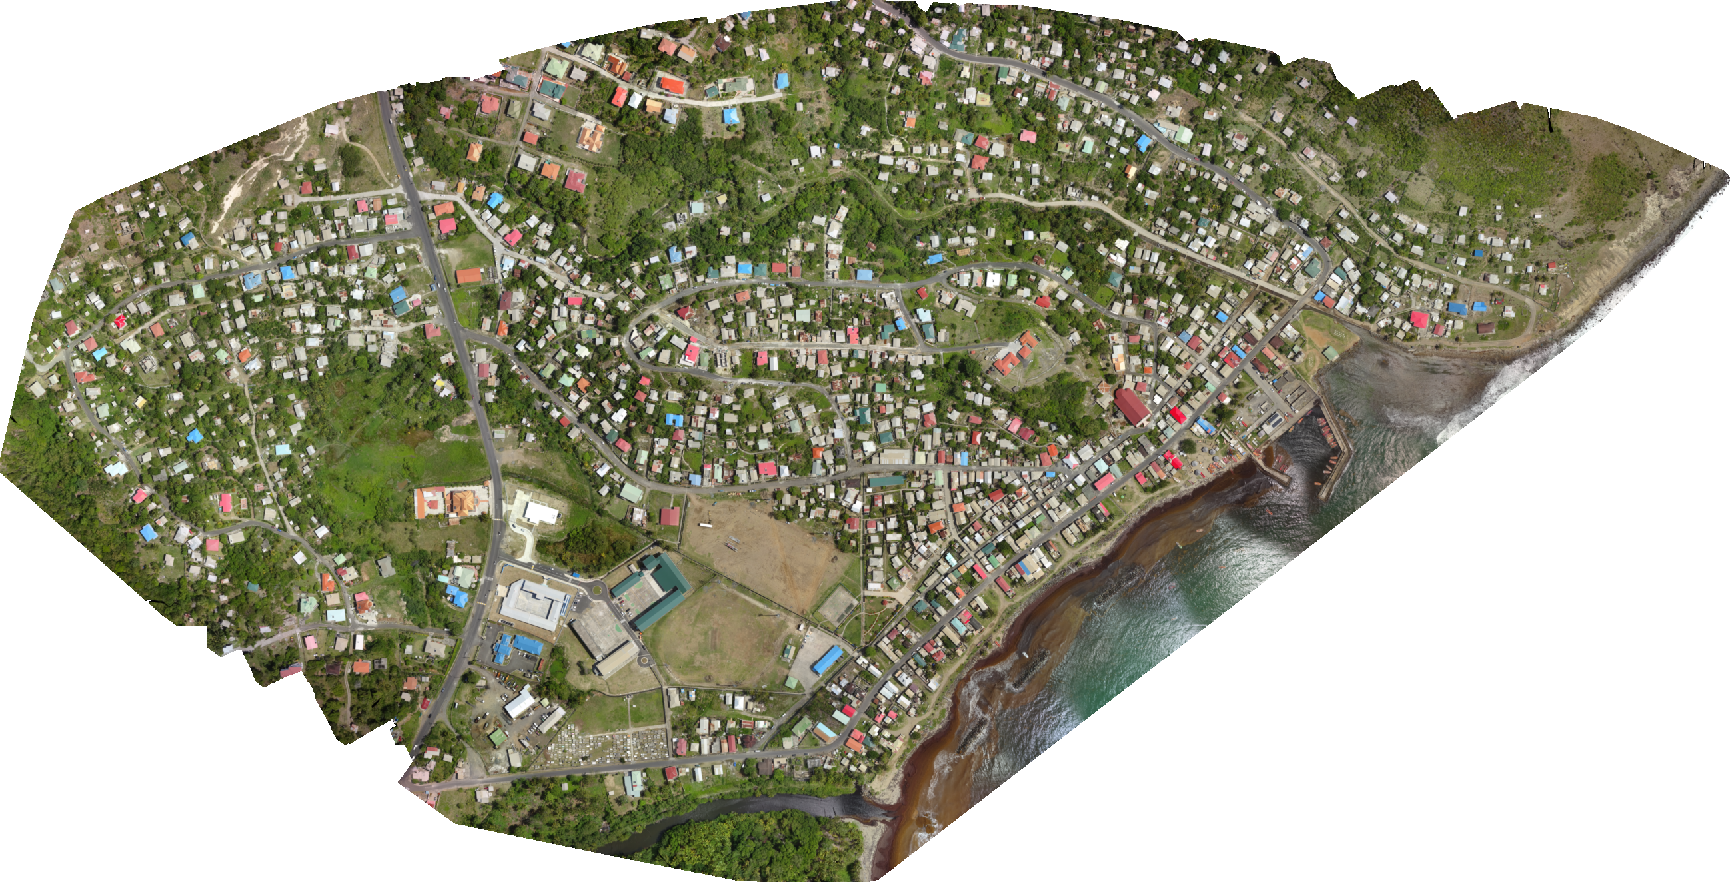
\includegraphics[width=0.7\textwidth]{figures/thumbnail_dennery.png}
		\caption{Thumbnail of stitched drone image from Dennery, St.Lucia.}
		\label{fig:thumbnail_dennery}
	\end{figure}

	The data provided for the challenge consists of high resolution ($\sim4$cm) drone imagery of five patches of land: two from Soacha, Colombia, two from Mixco, Guatemala and one from Dennery (St. Lucia).
	For every region, there is one stitched cloud-optimized GeoTIFF file, ranging from 500 to 1800 Megapixels in size. A thumbnail of the Dennery settlement is shown as example in Fig.~\ref{fig:thumbnail_dennery}.\\
	General information about the images is summarized in table~\ref{tab:general}.

	\begin{center}
		\bgroup
		\def\arraystretch{1.1}
		\begin{tabular}{ | m{5cm} | m{10cm}|} 
			\hline
			Platform & WeRobotics (private drone)  \\ 
			\hline
			Source & DrivenData Competition \newline https://www.drivendata.org/competitions/58/disaster-response-roof-type/data/ \\ 
			\hline
			Acquisition Method & Drone Photography  \\ 
			\hline
			SRS  & Ellipsoid (EPSG:32616, 32618, 326120)  \\ 
			\hline
			Spatial/Spectral resolution & 3.8-4.5cm, RGB  \\ 
			\hline
			Type of Product & Cloud-optimized GeoTIFF \\ 
			\hline
		\end{tabular}
		\egroup		
		\captionof{table}{General information about provided data.} 
		\label{tab:general}
	\end{center}
	
	\subsection{Labels}
	Roofs are labeled as one of five classes, examples of which are given in Fig.~\ref{fig:mat_examples}. The footprints of roofs are provided for both training and test set, i.e. roof segmentations are always given. There is a total of 14852 training examples, which are highly unbalanced throughout the classes.
	The log-loss as score for the \textit{Open AI Challenge} was computed on 7320 test images, for which class membership probabilities needed to be calculated.
	
	\begin{enumerate}
		\itemsep0em
		\item Concrete and Cement (1385 training samples): Roofs made out of concrete or cement.
		\item Healthy Metal (7370): Roofs of metal that are intact but may be corrugated or galvanized.
		\item Incomplete (668): Roofs that are severely damaged or under construction.
		\item Irregular Metal (5236): Roofs that are slightly damaged, rusted or patched.
		\item Other (193): Roofs that do not fit into other categories (include tiles, red painted, other materials).
	\end{enumerate}

	\begin{figure}
		
		\centering
		\begin{subfigure}[c]{0.32\textwidth}
			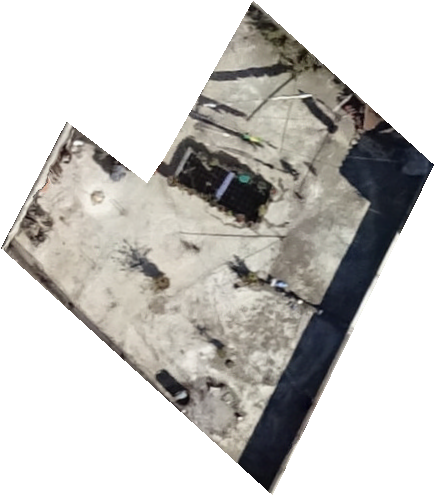
\includegraphics[width=0.47\textwidth]{figures/mat_examples/conc1.png}		
			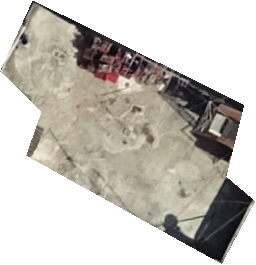
\includegraphics[width=0.47\textwidth]{figures/mat_examples/conc2.png}
			\subcaption{Concrete/Cement}
		\end{subfigure}
		\begin{subfigure}[c]{0.32\textwidth}
			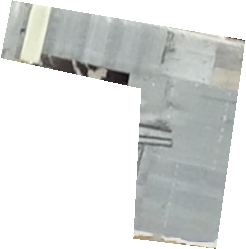
\includegraphics[width=0.47\textwidth]{figures/mat_examples/hm1.png}		
			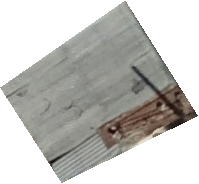
\includegraphics[width=0.47\textwidth]{figures/mat_examples/hm2.png}
			\subcaption{Healthy Metal}
		\end{subfigure}
		\begin{subfigure}[c]{0.32\textwidth}
			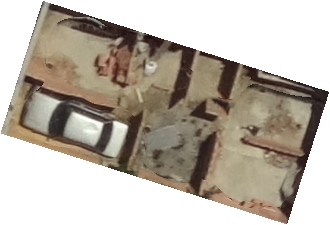
\includegraphics[width=0.47\textwidth]{figures/mat_examples/inc1.png}		
			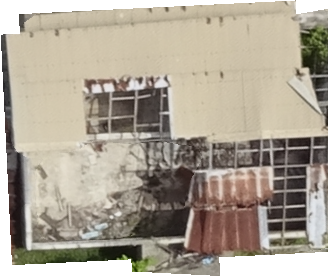
\includegraphics[width=0.47\textwidth]{figures/mat_examples/inc2.png}
			\subcaption{Incomplete}
		\end{subfigure}
		\begin{subfigure}[c]{0.32\textwidth}
			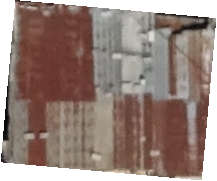
\includegraphics[width=0.32\textwidth]{figures/mat_examples/irr1.png}		
			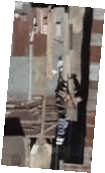
\includegraphics[width=0.32\textwidth]{figures/mat_examples/irr2.png}
			\subcaption{Irregular Metal}
		\end{subfigure}
		\begin{subfigure}[c]{0.32\textwidth}
			\centering
			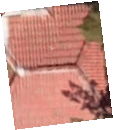
\includegraphics[width=0.35\textwidth]{figures/mat_examples/other1.png}		
			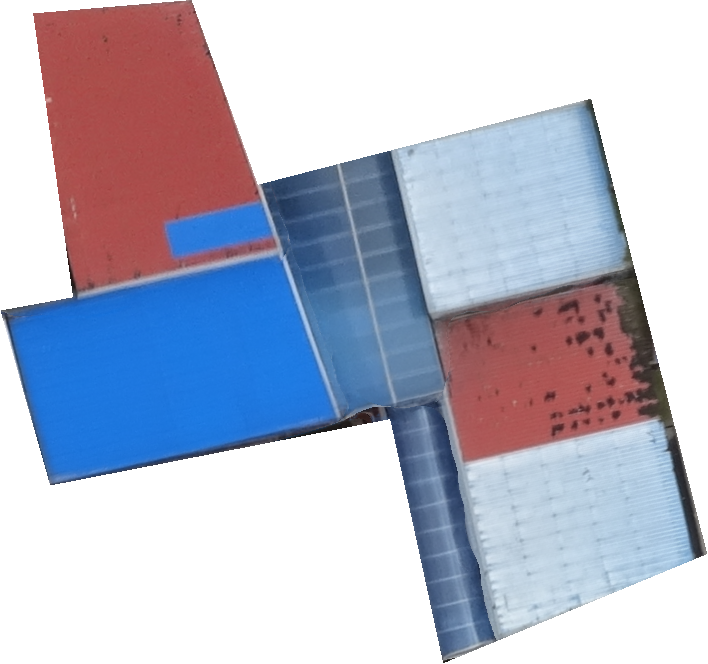
\includegraphics[width=0.45\textwidth]{figures/mat_examples/other2.png}
			\subcaption{Other}
		\end{subfigure}
	\caption{Example images for each material class. (Scales differ)}
	\label{fig:mat_examples}
	\end{figure}

	\subsection{Data Noise}
	
	Unfortunately, class membership is sometimes ambiguous in the provided groundtruth data. 
	First, labels are used inconsistently. This is especially true for "irregular" and "healthy metal". Where rusty roofs should be labeled as "irregular", many of them get a "healthy metal" label.
	Moreover there is confusion about properties that make a roof "irregular" or "incomplete".
	These inconsistencies might stem from different annotators labeling images.
	
	Second, labels are sometimes clearly incorrect, e.g. concrete roofs are labeled as "healthy metal". In that regard, some regions seem to be annotated with more care than others. 
	
	It is impossible to quantify the extent to which annotations are noisy. 
	Some examples of these ambiguities are shown in Fig.~\ref{fig:ambiguities}.
	The implications for the results are discussed in section~\ref{sec:discussion}.
	
	\begin{figure}
		\centering
		\begin{subfigure}[c]{0.27\textwidth}
			\centering
			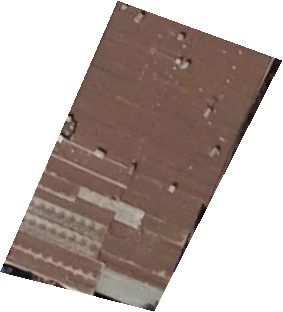
\includegraphics[width=.72\textwidth]{figures/wrong_labels/hm_rusty.png}
			\subcaption{"healthy metal"}	
		\end{subfigure}	
		\begin{subfigure}[c]{0.27\textwidth}
			\centering
			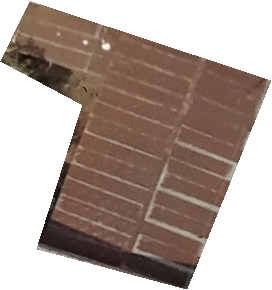
\includegraphics[width=.72\textwidth]{figures/wrong_labels/irr_rusty.png}
			\subcaption{"irregular metal"}
		\end{subfigure}
		\begin{subfigure}[c]{0.27\textwidth}
			\centering
			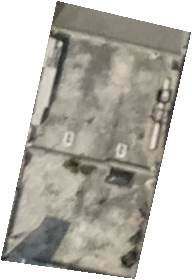
\includegraphics[width=.9\textwidth]{figures/wrong_labels/hm_should_be_conc.png}
			\subcaption{Labeled "irregular metal" where clearly concrete}
		\end{subfigure}
		\vspace{.3cm}]
		\begin{subfigure}[c]{0.35\textwidth}
			\centering
			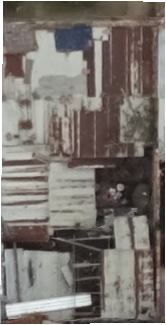
\includegraphics[width=0.67\textwidth]{figures/wrong_labels/irr_holes.png}
			\subcaption{Labeled "irregular metal"}
		\end{subfigure}
		\begin{subfigure}[c]{0.35\textwidth}
			\centering		
			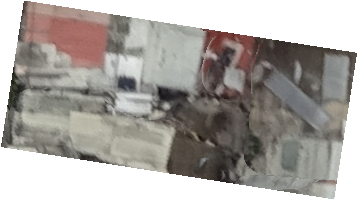
\includegraphics[width=0.72\textwidth]{figures/wrong_labels/inc_holes.png}
			\subcaption{Labeled "incomplete"}
		\end{subfigure}
		\caption{(a) and (b) named differently due to incoherent labeling of rusty roofs. Similarly unclear boundary between "irregular metal" and "incomplete" ((d) and (e)). Obvious labeling error in (c).}
		\label{fig:ambiguities}
	\end{figure}

	
	\section{Proposed Processing Routine}
	
	\subsection{Petrained Neural Network as Feature Extractor}		
	
	The proposed processing routine uses a pretrained neural network as feature extractor. Different publicly available architectures were tested, such as ResNet50~\cite{resnet}, InceptionV3~\cite{inceptionv3}, DenseNet201~\cite{densenet} and VGG16~\cite{vgg}. The employed pretrained architectures were trained on more than a million images of 1000 categories from the ImageNet database ~\cite{imagenet}. 
	ImageNet is a collection of natural images of common objects and animals. The features which are relevant to distinguish those classes, are very likely also relevant to discriminate other types of natural images, such as roofs.
	In order to obtain features, the classification layer is removed and replaced by an average or maximum pooling layer to reduce the number of features.\\	
	
	In the next step, a Support Vector Machine (SVM) or Random Forest (RF) is trained to classify roof materials based on the extracted features. The calculated classification can then be used to predict class membership based on features of test samples. For the context of the challenge, prediction probabilities needed to be calculated. The \textit{scikit-learn} implementation of both SVM and RF provide pseudo-probabilities that take a samples' distance to the decision boundary into account. Those probabilities/confidences were submitted for evaluation on the challenge website.
	The full classification pipeline is presented in Fig.~\ref{fig:flowchart}.
	
	
	\begin{figure}
		\centering		
		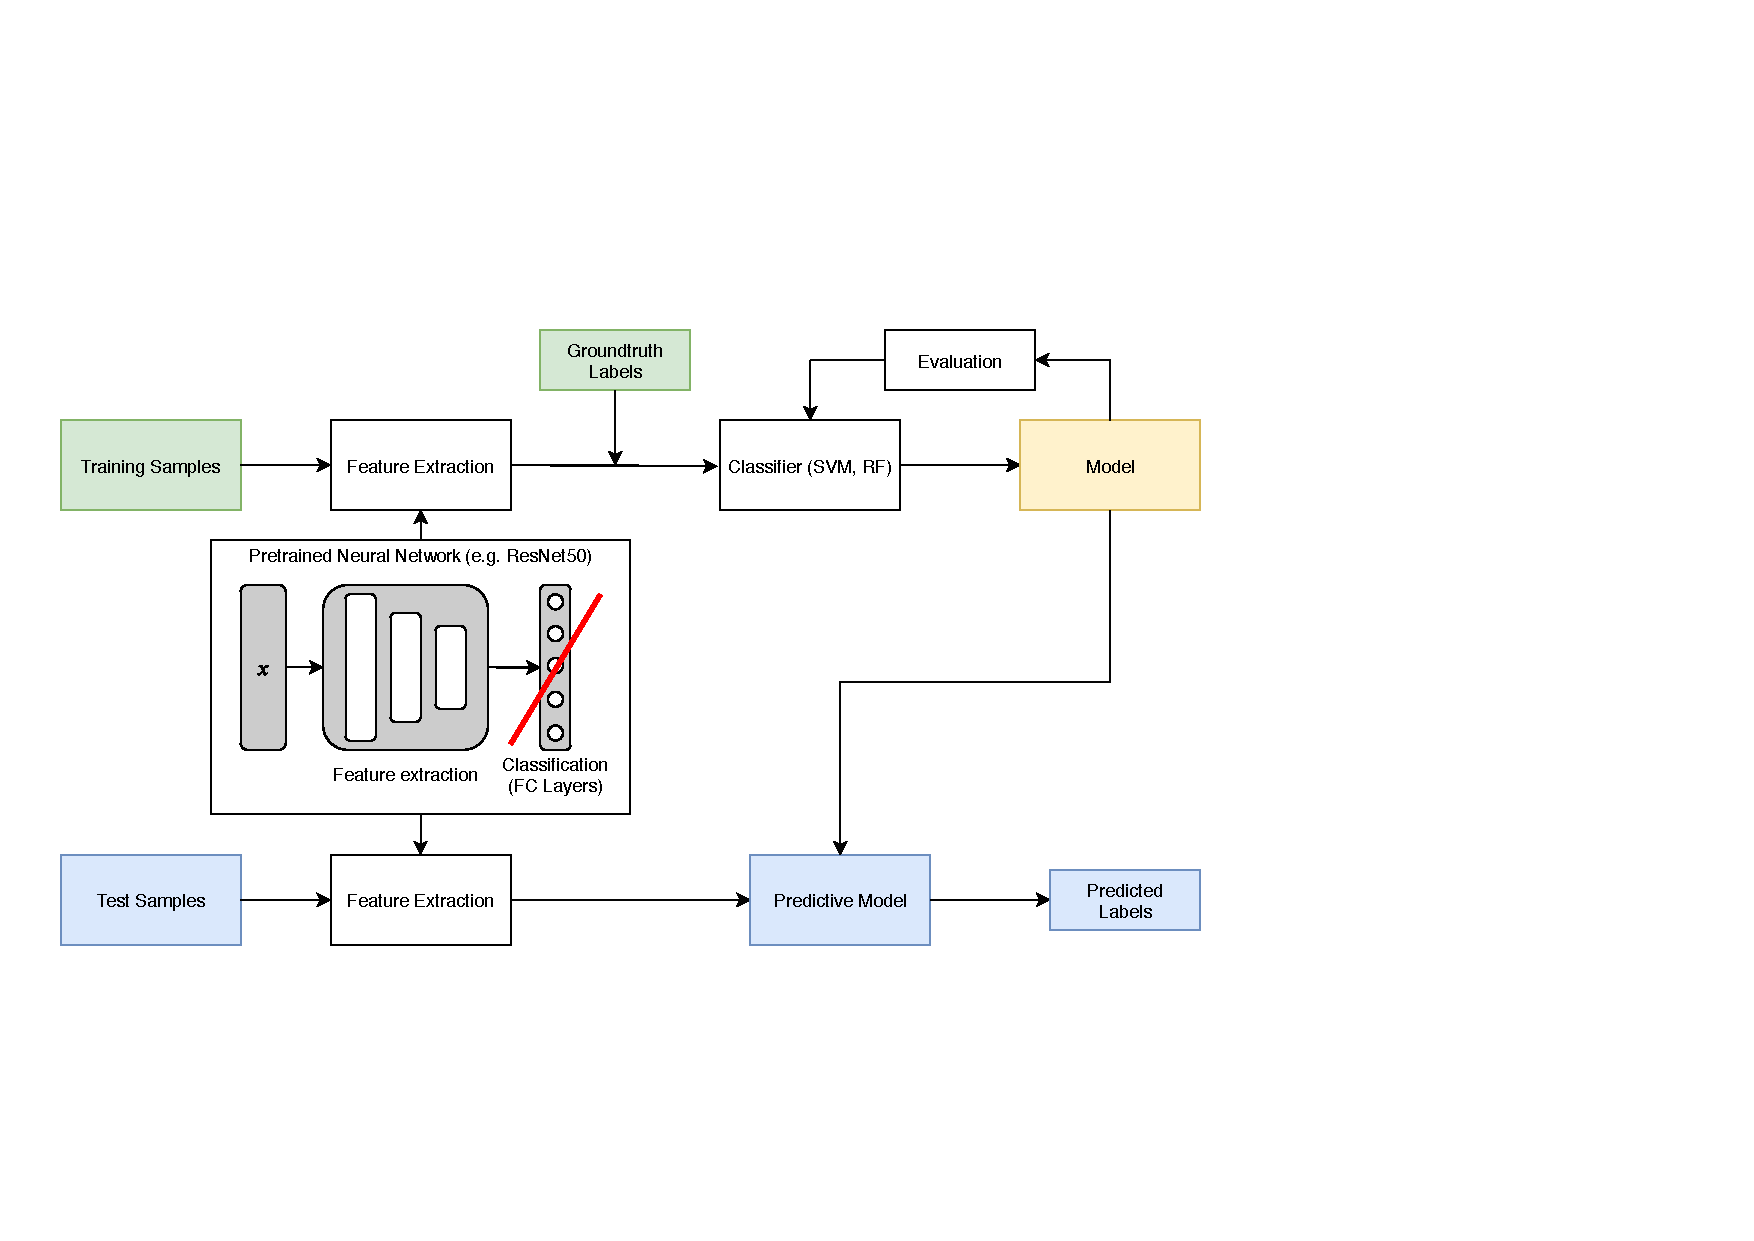
\includegraphics[width=0.8\textwidth]{figures/flowchart.pdf}
		\caption{Proposed processing routine: The classification part of a pretrained neural network is removed, leaving the feature extraction. A SVM or RF is used to build a model out of the training features and the groundtruth labels in an iterative process. Test features are fed into this model to predict labels and determine prediction confidence.}
		\label{fig:flowchart}
	\end{figure}

	\subsection{Pixel-based Baseline } 
	\label{sec:pixel_based}
	As a baseline for comparison, several statistical metrics are extracted as features and classified with a SVM. The mean is used to assess the dominant colors on a roof. Heterogeneity is tried to measure using the standard deviation and range of every image. Every metric is calculated on every color channel and on the absolute of the Sobel-filtered image in x- and y-direction of every color channel (see Fig.~\ref{fig:pixel_based}). This results in a 18-dimensional feature vector (3 metrics $\times$ 3 channels on original and gradient image).
	
	\begin{figure}
		\centering
		\begin{subfigure}[t]{\textwidth}
			\centering
			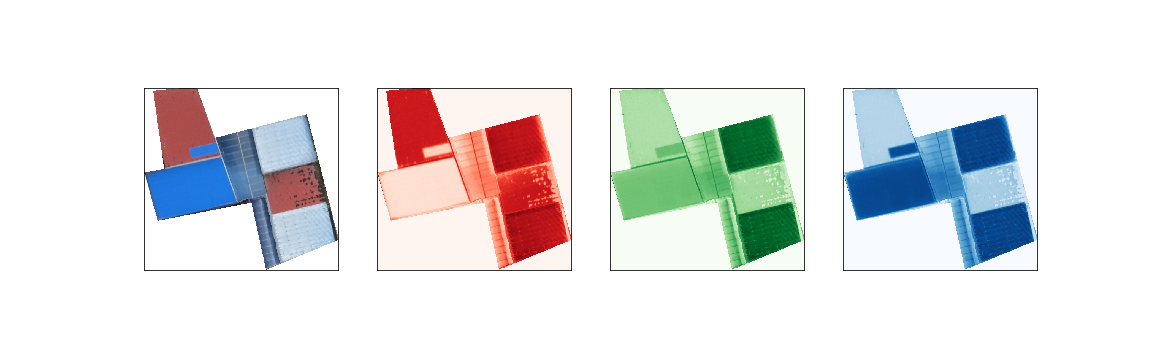
\includegraphics[width=\textwidth, trim={3cm 3cm 3cm 3cm},clip]{figures/pixel_based/rgb_channels.png}
			\subcaption{RGB Image and individual color channels}
		\end{subfigure}
		\begin{subfigure}[b]{.8\textwidth}
			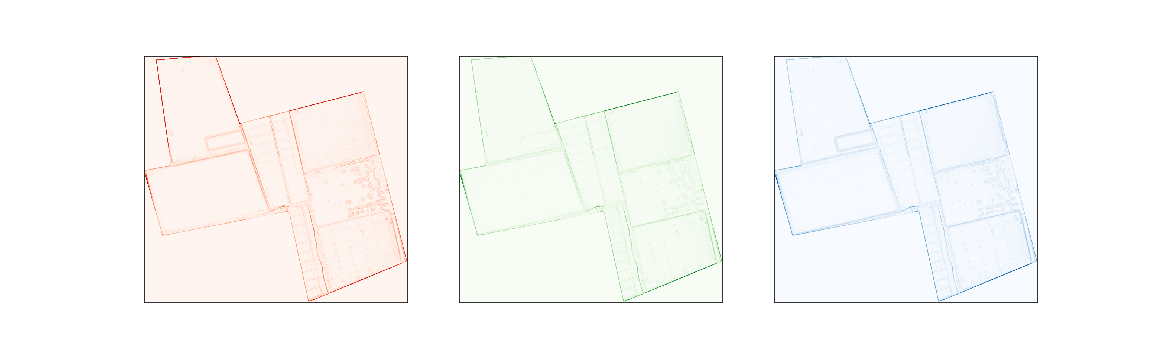
\includegraphics[width=.95\textwidth, trim={2cm 1.5cm 2cm 1.5cm},clip]{figures/pixel_based/sobel.png}
			\subcaption{Derivative images (absolute of Sobel-filtered images in x- and y-direction)}
		\end{subfigure}
		\caption{Original image classified as "other" with red, green and blue individual channels (top row). \\ Gradient images of each channel (bottom row)}
		\label{fig:pixel_based}
	\end{figure}
	
	\section{Results}
	
	Before investigating results it has to be clarified that the performance of the suggested system was optimized to perform well in the described \textit{Open AI challenge}. The predictions to be submitted were class membership probabilities and not hard labels. Since the algorithm is supposed to just hint at high risk roofs to be revisited by a human instructor instead of indicating one clear action, this seems reasonable. In section~\ref{sec:challenge_perf}, the challenge performance is presented. Section~\ref{sec:class_comparison} shows results that used only the training data to compare the system to other classifiers using more metrics.
	
	\subsection{Online Challenge Performance}
	\label{sec:challenge_perf}
	
	For the \textit{Open AI challenge}, system performance was evaluated using the log loss:
	
	\begin{equation}
		loss = -\frac{1}{N}\cdot \sum_{i=1}^{N} \sum_{j=1}^{M}y_{ij}\log p_{ij}
	\end{equation}
	
	In that context, $N$ was the number of test samples (=7320), $M$ the number of classes (=5), $y_{ij}$ the true label, i.e. 1 if observation $i$ belonged to class $j$ and 0 otherwise and $p_ij$ was the predicted probability that $i$ was of class $j$. 
	
	The best-performing setup consisted of a ResNet50 as feature extractor with average pooling at the end and classification using a SVM with a high regularization parameter $C=100$.
	Other pretrained networks performed similarly well, although not quite as good. Results on the test in terms of log-loss are shown in table~\ref{tab:model_comparison}.
	The top score of 0.5554 corresponded to rank 51 in a field of 1425 competitors (top 4\%).
	
	\begin{center}
		\bgroup
		\def\arraystretch{1.1}
		\begin{tabular}{ | m{4cm} | m{2cm} | } 
			
			\hline
			Pretrained model & Log-loss \\
			\hline
			\hline
			ResNet50 & 0.5554 \\
			\hline
			InceptionV3 & 0.5917\\
			\hline
			DenseNet201 & 0.5800\\
			\hline
			VGG16 & 0.6152\\
			\hline
		\end{tabular}
		\egroup
		\captionof{table}{Log-loss on online challenge test set for feature extraction with different pretrained models. Classification was always performed with an SVM using $C=100$.} 
		\label{tab:model_comparison}
	\end{center}

	
	\subsection{Removing Noisy Labels}
	The problem of noisy data was tried to be tackled by selecting clean subsets of training data to improve the accuracy of the model. However in terms of log-loss on the test set, this proved to be counterproductive. It is likely that due to more homogeneous training sets, the model became bad at handling noise (wrong or contentious labels) and was punished heavily for "wrong" classifications with high confidence.
	
	\subsection{Comparing Performances}
	\label{sec:class_comparison}
	Since classification performance measures require groundtruth data, the previously so-called "training set" provided for the challenge was split into new training and test sets for the evaluation.
		
	To assess the difficulty of the task and the improvement through features extracted by neural networks, the system performance was compared against the pixel-based approach described in section~\ref{sec:pixel_based}.
	Moreover, the Support Vector Machine as the best-performing classifier was tested against a Random Forest model. For both classification methods, parameters were empirically optimized. For SVM a value of $C=100$ was found to work well. As for RF, 1000 trees were trained with a maximum depth of 16. 
	%Computation times for classifier training increases drastically with the amount of considered features. Furthermore, eliminating irrelevant features can improve classification. Feature importance can be easily ranked...
	
	\begin{center}
		\bgroup
		\def\arraystretch{1.1}
		\begin{tabular}{ | m{5cm} | m{2cm} | m{2cm} | m{2cm} |} 
			
			\hline
			Method & Avg. Log-loss & Avg. Accuracy & Avg. Macro-F1 \\
			\hline
			\hline
			Pixel-based features + SVM & 0.82 & 0.68 & 0.49  \\
			\hline
			Pixel-based features + RF & 0.80 & 0.68 & 0.38  \\
			\hline
			ResNet50 + SVM & 0.57 & 0.76 & 0.63 \\
			\hline
			ResNet50 + RF & 0.70 & 0.75 & 0.45  \\
			\hline
		\end{tabular}
		\egroup
		\captionof{table}{Performance metrics of best-performing pixel-based and suggested processing routines. (Note, that a lower log-loss indicates a better result)} 
		\label{tab:pb_vs_nn}
	\end{center}
	
	The significant improvement in performance from pixel-based to deep features also becomes visible in ~\ref{fig:pixel_based_cm}. It shows the confusion matrices for both classifiers using a random split. When visually assessing the result, the class imbalances should be kept in mind. Only 4.5\% of the roofs carry the true label "incomple", 1.3\% "other". It becomes apparent that both classifiers struggle to identify the least represented classes correctly.
	
	\begin{figure}
		\begin{subfigure}[t]{.5\textwidth}
			\centering
			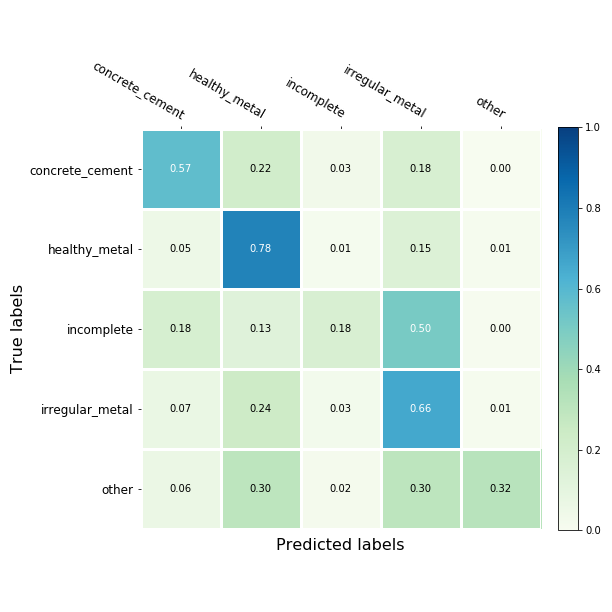
\includegraphics[width=0.9\textwidth]{figures/results/pixel_based_cm.png}
			\caption{Pixel-based features classified by SVM}
		\end{subfigure}
		\begin{subfigure}[t]{.5\textwidth}
			\centering
			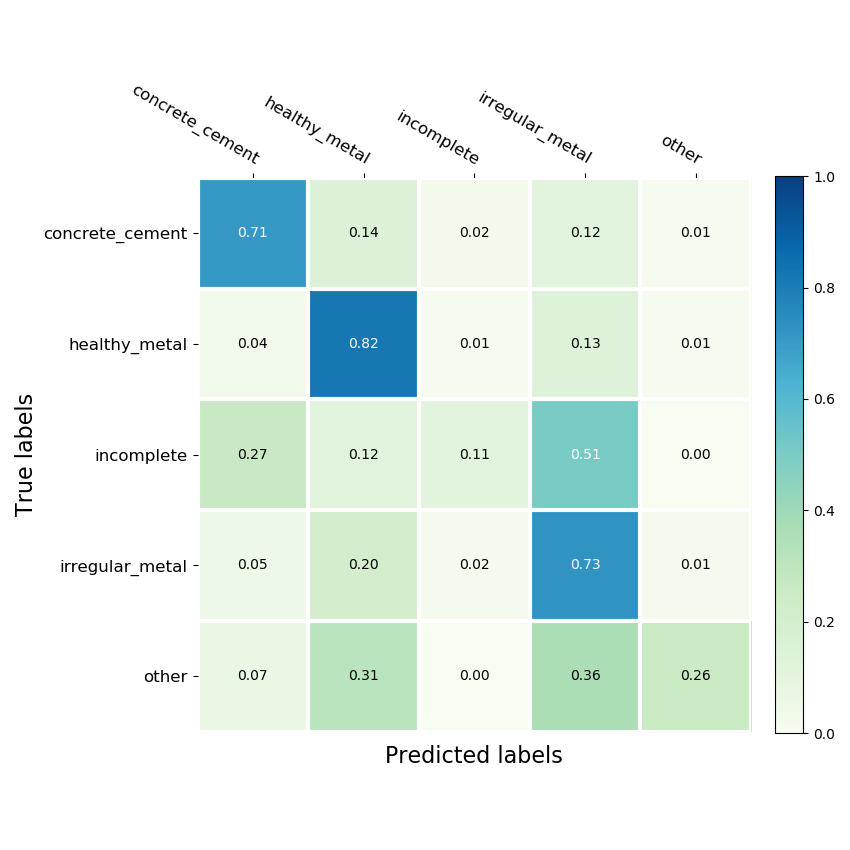
\includegraphics[width=0.9\textwidth]{figures/results/nn_based_cm.png}
			\caption{ResNet50 features classified by SVM}
		\end{subfigure}
	\caption{Confusion Matrices for pixel-based vs. deep features on random split of the provided data (same split for both).}
	\label{fig:pixel_based_cm}
	\end{figure}
	
	Map with colored rectangles indicating roof security?????????????
	
	
	\section{Discussion}
	\label{sec:discussion}
	
	Comment on confusion matrices
	
	Comment on class imbalance
	
	
	Discussion where you are critical about what has been done and what could be further explored. You have investigated a topic and achieving your initial goal is not always possible in a fixed time frame, however you should be able to assess your situation and what should then be done/improved in order to reach your goal.
	
	\subsection{Outlook}
	Outlook: Retrain network
	
	Assess the "real performance" by cleaning up the noisy data
	
	\section{Appendix}

	The used code is publicly accessible on GitHub, mostly in the form of Jupyter Notebooks \\
	(see \url{https://github.com/jo-ruether/ipeo_carribean}).
	
	
	\bibliography{ipeo} 
	\bibliographystyle{ieeetr}

\end{document}